
%(BEGIN_QUESTION)
% Copyright 2008, Tony R. Kuphaldt, released under the Creative Commons Attribution License (v 1.0)
% This means you may do almost anything with this work of mine, so long as you give me proper credit

In this automotive fuel level sensing circuit, a current mirror is supposed to maintain a constant current (about 25 to 26 mA) through the fuel level sensor, which is nothing more than a variable resistance (rheostat) that changes with fuel level.  The voltage dropped across this sensor resistance is then sent to a fuel gauge: a voltmeter with the scale calibrated in gallons of fuel level:

$$\includegraphics[width=15.5cm]{i03185x01.eps}$$

There is a problem in this circuit, though.  The fuel gauge reads empty even when you know the fuel tank is completely full.  You take two DC voltage measurements to begin your troubleshooting: +12 volts between TP2 and ground, and 0 volts between TP3 and ground.

From this information, identify two possible faults (either one of which could account for the problem and all measured values in this circuit), and also identify two circuit elements that could not possibly be to blame (i.e. two things that you know {\it must} be functioning properly, no matter what else may be faulted).  The circuit elements you identify as either possibly faulted or properly functioning can be wires, traces, and connections as well as components.  Be as specific as you can in your answers, identifying both the circuit element and the type of fault.

\medskip
\goodbreak
\item{} Circuit elements that are possibly faulted
\item{1.}
\item{2.} 
\end{itemize}

\medskip
\goodbreak
\item{} Circuit elements that must be functioning properly
\item{1.} 
\item{2.} 
\end{itemize}

\vfil 

\underbar{file i03185}
\eject
%(END_QUESTION)





%(BEGIN_ANSWER)

This is a graded question -- no answers or hints given!

%(END_ANSWER)





%(BEGIN_NOTES)

The 0 volt measurement at TP3 is not good, because we ordinarily should see voltage as a result of the constant (regulated) current passing through the resistance of the fuel level sensor.  The 12 volt measurement at TP2 is also abnormal, as we should normally expect transistor Q1 to drop approximately 0.7 volts as it performs its function of a diode (a simple PN junction).  

\vskip 10pt

The problem, therefore, appears to lie within the current mirror circuit, causing it to output zero current to the fuel level sensor, and therefore cause the fuel gauge to register empty.  Specifically, the problem appears to lie with the Q1/R1 half of the current mirror, given the 12 volt measurement at TP2.

\vskip 10pt

\begin{itemize}
\item{} Circuit elements that are possibly faulted
\item{1.} Transistor $Q_1$ failed shorted
\item{2.} Resistor $R_1$ failed open
\end{itemize}

\begin{itemize}
\item{} Circuit elements that must be functioning properly
\item{1.} Ignition switch
\item{2.} Battery
\end{itemize}

%INDEX% Troubleshooting review: electric circuits

%(END_NOTES)


